\documentclass[../main.tex]{subfiles}
\begin{document}

\section{Metodología}
En este capítulo se describe con detalle la metodología seguida para el desarrollo del sistema de segmentación automática de lesiones de esclerosis múltiple. Primero, se presenta el conjunto de datos utilizado y el proceso de preprocesado necesario para convertir las imágenes volumétricas originales en cortes bidimensionales adecuados para el entrenamiento de redes neuronales. A continuación, se explican los criterios de división del conjunto de datos, incluyendo la adopción de una estrategia de validación cruzada para una evaluación más robusta.

Seguidamente, se describe el flujo completo de preprocesado, desde la lectura de las imágenes hasta su adaptación al formato requerido por cada modelo. Posteriormente, se detallan las distintas estrategias de selección de imágenes evaluadas en el trabajo, diseñadas para estudiar el impacto que tiene la composición del conjunto de entrenamiento en el rendimiento del sistema.

Finalmente, se enumeran y definen las métricas utilizadas para cuantificar la calidad de las segmentaciones obtenidas, abarcando tanto medidas de solapamiento espacial como de rendimiento computacional. Esta metodología proporciona un marco experimental sólido para comparar las diferentes configuraciones propuestas a lo largo del estudio.

\subsection{Enfoque experimental}
El objetivo principal es desarrollar un sistema automático capaz de segmentar de forma precisa las lesiones provocadas por la esclerosis múltiple en imágenes de resonancia magnética cerebral. Este sistema busca facilitar la labor de diagnóstico y seguimiento de pacientes, reduciendo la carga de trabajo de los profesionales sanitarios y aumentando la objetividad del proceso.

Para abordar este reto, se ha planteado una metodología experimental basada en la comparación de múltiples configuraciones, que combinan diferentes arquitecturas de red, estrategias de selección de imágenes y técnicas de mejora de resolución. En concreto, se han evaluado los siguientes factores:

\begin{itemize}
    \item \textbf{Arquitectura:} se han utilizado dos modelos de segmentación, U-Net y YOLO.
    \item \textbf{Selección de slices:} se han diseñado tres estrategias con el fin de comparar las redes.
    \item \textbf{Super-resolución:} se ha evaluado el impacto de aplicar un modelo FSRCNN para duplicar la resolución espacial de las imágenes antes del entrenamiento.
\end{itemize}

La combinación de estas variantes da lugar a un conjunto de diez experimentos distintos, que se enumeran en la Tabla~\ref{tab:experimentos}. \textbf{Lesión} se refiere a la inclusión exclusiva de cortes con una región lesionada, \textbf{Cerebro} selecciona cortes con o sin lesion pero no vacíos, \textbf{$\times 2$} indica la aplicación de super-resolución. Cada configuración ha sido evaluada utilizando un conjunto de métricas estándares para segmentación médica, con el objetivo de identificar cuál de ellas ofrece el mejor equilibrio entre precisión y robustez.

\begin{table}[h]
\centering
\caption{Resumen de las configuraciones experimentales evaluadas.}
\label{tab:experimentos}
\begin{tabular}{cccccc}
\toprule
\textbf{ID} & \textbf{Red} & \textbf{Selección de Slices} & \textbf{Super-resolución} \\
\midrule
A & U-Net & Base                    & Sin SR \\
B & YOLO  & Base                    & x2     \\
C & U-Net & Base                    & x2     \\
D & YOLO  & Base                    & Sin SR \\
E & U-Net & Lesión                  & Sin SR \\
F & U-Net & Lesión                  & x2     \\
G & YOLO  & Lesión                  & Sin SR \\
H & YOLO  & Lesión                  & x2     \\
I & U-Net & Cerebro                 & Sin SR \\
J & U-Net & Cerebro                 & x2     \\
K & YOLO  & Cerebro                 & Sin SR \\
L & YOLO  & Cerebro                 & x2     \\
\bottomrule
\end{tabular}
\end{table}

En las siguientes secciones se describen con mayor detalle el conjunto de datos utilizado, los procesos de preprocesamiento y selección de imágenes, así como las métricas empleadas para la evaluación de los modelos.

\subsection{Conjunto de datos y preprocesado}
El conjunto de datos utilizado es el \textit{MSLesSeg-Dataset}, proporcionado en el contexto de la competición internacional \textit{ICPR 2024} (\textit{International Conference on Pattern Recognition}). Estos datos han sido diseñados específicamente para avanzar en el desarrollo de sistemas completamente automáticos de segmentación de lesiones de esclerosis múltiple, y destaca por su amplitud, calidad de anotaciones y realismo clínico. El conjunto está compuesto por imágenes de resonancia magnética de 75 pacientes reales diagnosticados con EM, obtenidas en condiciones clínicas habituales. Cada paciente cuenta con entre uno y cinco puntos temporales de seguimiento. Para cada uno de estos puntos temporales, se incluyen tres modalidades de imagen: T1-weighted (T1-w), T2-weighted (T2-w) y FLAIR. Las máscaras de segmentación de las lesiones han sido generadas manualmente por expertos a partir de las secuencias FLAIR, que son las más sensibles para la detección de lesiones de EM. Las modalidades T1-w y T2-w también se proporcionan para favorecer una caracterización multimodal más completa de las lesiones. De los 75 pacientes, hay 22 pacientes que no disponen de máscaras de segmentación. Por lo tanto, se han descartado todas sus imágenes por completo. El resto de pacientes, 53, sí disponen de máscaras de segmentación y sus imágenes han sido usadas en este trabajo.

En cuanto al formato de las imágenes, están en formato NIfTI (\textit{Neuroimaging Informatics Technology Initiative}), un estándar ampliamente utilizado en neuroimagen médica para almacenar datos volumétricos tridimensionales. En el caso de las imágenes de \textit{MSLesSeg-Dataset}, presentan unas dimensiones $182 \times 218 \times 182$ en los ejes $X$, $Y$, y $Z$, respectivamente. Los valores de intensidad están almacenados en coma flotante (\textit{float64}). Este formato almacena un volumen tridimensional de intensidades, habitualmente compuesto por cortes adquiridos en un plano específico (ej. axial), Figura \ref{fig:nifti-ejes}.

\begin{figure}
    \centering
    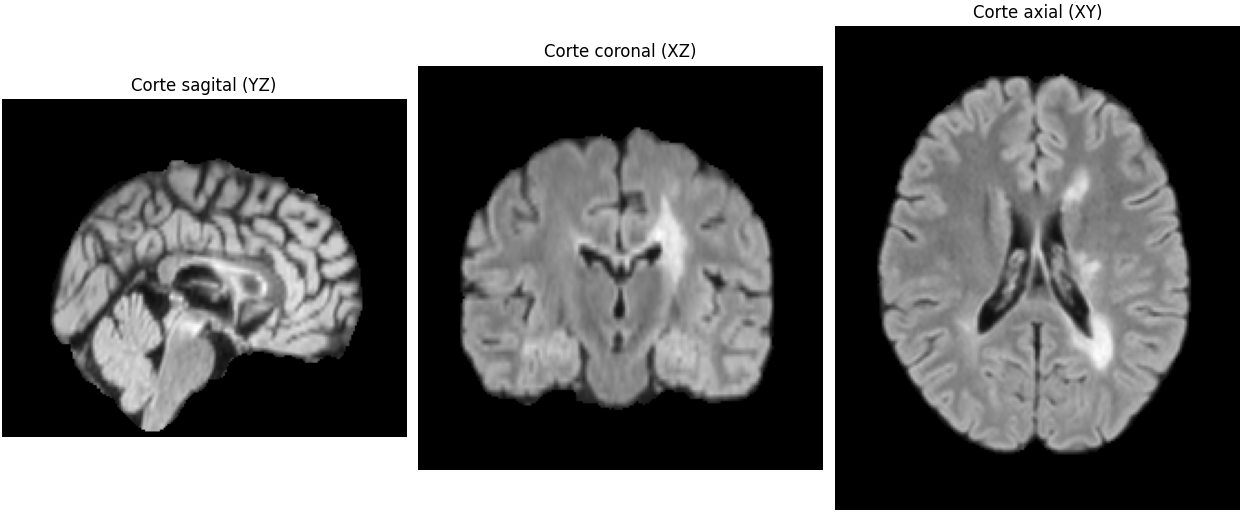
\includegraphics[width=0.7\linewidth]{imgs/metodologia/nifti1.png}
    \caption{Visualización de los tres planos anatómicos principales a partir de un volumen FLAIR en formato NIfTI. De izquierda a derecha: corte sagital (vista lateral del cerebro), corte coronal (vista frontal) y corte axial (vista desde arriba). Cada imagen corresponde a un corte central extraído a lo largo del eje correspondiente del volumen tridimensional.}
    \label{fig:nifti-ejes}
\end{figure}

En este trabajo se ha optado por utilizar cortes axiales ($XY$) como base para el preprocesado y entrenamiento de los modelos. Esta elección se debe a que los volúmenes del dataset original están organizados naturalmente en ese plano, lo que significa que cada corte axial corresponde a un corte adquirido directamente por el escáner de resonancia magnética. Trabajar en este plano garantiza que los modelos trabajen sobre datos que reflejan la resolución y geometría originales del estudio, evitando interpolaciones innecesarias en los ejes reconstruidos. Además, Como el objetivo es predecir las regiones lesionadas según las máscaras de referencia, y estas han sido definidas visualmente sobre la secuencia FLAIR (donde las lesiones se ven claramente), se ha optado por entrenar el modelo únicamente con las imágenes FLAIR. Esto asegura que el modelo aprenda a segmentar a partir de la fuente de información más directa y coherente con las anotaciones manuales.

\subsection{División del conjunto de datos}
En una fase inicial del trabajo, se optó por una división clásica del conjunto de datos, compuesto por 53 pacientes, en tres subconjuntos independientes: entrenamiento (\textit{train}), validación (\textit{val}) y prueba (\textit{test}). Esta estructura permitió entrenar los modelos con un conjunto de datos amplio, ajustar los hiperparámetros utilizando el conjunto de validación y evaluar el rendimiento final sobre un conjunto de prueba completamente separado. Esta estrategia es habitual en muchos estudios y proporciona una línea base de evaluación clara y comprensible.

No obstante, considerando el número limitado de muestras disponibles (en especial dado que el conjunto de datos está formado por pacientes individuales, con un riesgo inherente de sobreajuste intrapaciente), se decidió posteriormente ampliar la evaluación mediante la incorporación de una estrategia de validación cruzada (\texttt{K-Fold Cross-Validation}). Esta técnica permite una estimación más robusta del rendimiento general del modelo, ya que cada muestra del conjunto de datos participa tanto en el entrenamiento como en la validación en diferentes iteraciones (\textit{folds}).

Concretamente, se empleó una validación cruzada estratificada con $K=5$, asegurando en cada \textit{fold} que no hubiera solapamiento de pacientes entre los conjuntos de entrenamiento y validación, lo cual es fundamental para evitar sesgos derivados de la correlación intrapaciente en las imágenes. A continuación, se resumen los tamaños de cada conjunto según la estrategia de selección de cortes utilizada:

\begin{itemize}
    \item \textbf{Base}: Se incluyeron todos los cortes disponibles. El número total de imágenes fue de 16744 (cuya distribución es de 9994 cortes vacíos y 6750 con lesión).
    \item \textbf{Base con superposición (x2)}: Mismo conjunto que el anterior, pero aplicando un modelo de super-resolución FSRCNN para duplicar la resolución espacial de las imágenes FLAIR. El número total de imágenes fue de 16744.
    \item \textbf{Lesión}: Se seleccionaron únicamente los cortes cuya máscara presentaba lesión. Esta configuración resultó en 6750 cortes.
    \item \textbf{Lesión con superresolución (x2)}: Misma selección que la anterior, aplicando además un aumento de resolución mediante un modelo FSRCNN.
    \item \textbf{Cerebro}: Se seleccionaron aquellos cortes que contuvieran cerebro. Es decir, se descartaron los cortes que no presentaban ninguna estructura cerebral visible aunque puedan no tener ninguna lesión. Esta selección resultó en 13563 cortes.
    \item \textbf{Cerebro con superresolución (x2)}: Misma selección anterior con aumento de resolución, manteniendo el mismo número de imágenes.
\end{itemize}

Se pueden distinguir varios tipos de cortes en función de su contenido:
\begin{itemize}
    \item \textbf{Cortes vacíos:} aquellos que no contienen ninguna estructura cerebral visible, ni lesión ni cerebro. Estos cortes no aportan información relevante para la segmentación y pueden introducir ruido en el entrenamiento del modelo.
    \item \textbf{Cortes con lesión:} aquellos que presentan al menos una región lesionada, independientemente de si también contienen otras estructuras cerebrales. Estos cortes son fundamentales para entrenar modelos de segmentación, ya que proporcionan ejemplos positivos de la clase objetivo.
    \item \textbf{Cortes con cerebro:} aquellos que contienen al menos una estructura cerebral visible, ya sea con o sin lesión. Estos cortes son útiles para entrenar modelos que deben aprender a segmentar el cerebro en general, no solo las lesiones.
\end{itemize}

A continuación se muestran dos figuras que ilustran la distribución de estos cortes.
\begin{figure}[H]
    \centering
    % Primera subfigura: valores absolutos
    \begin{subfigure}[b]{0.48\linewidth}
        \centering
        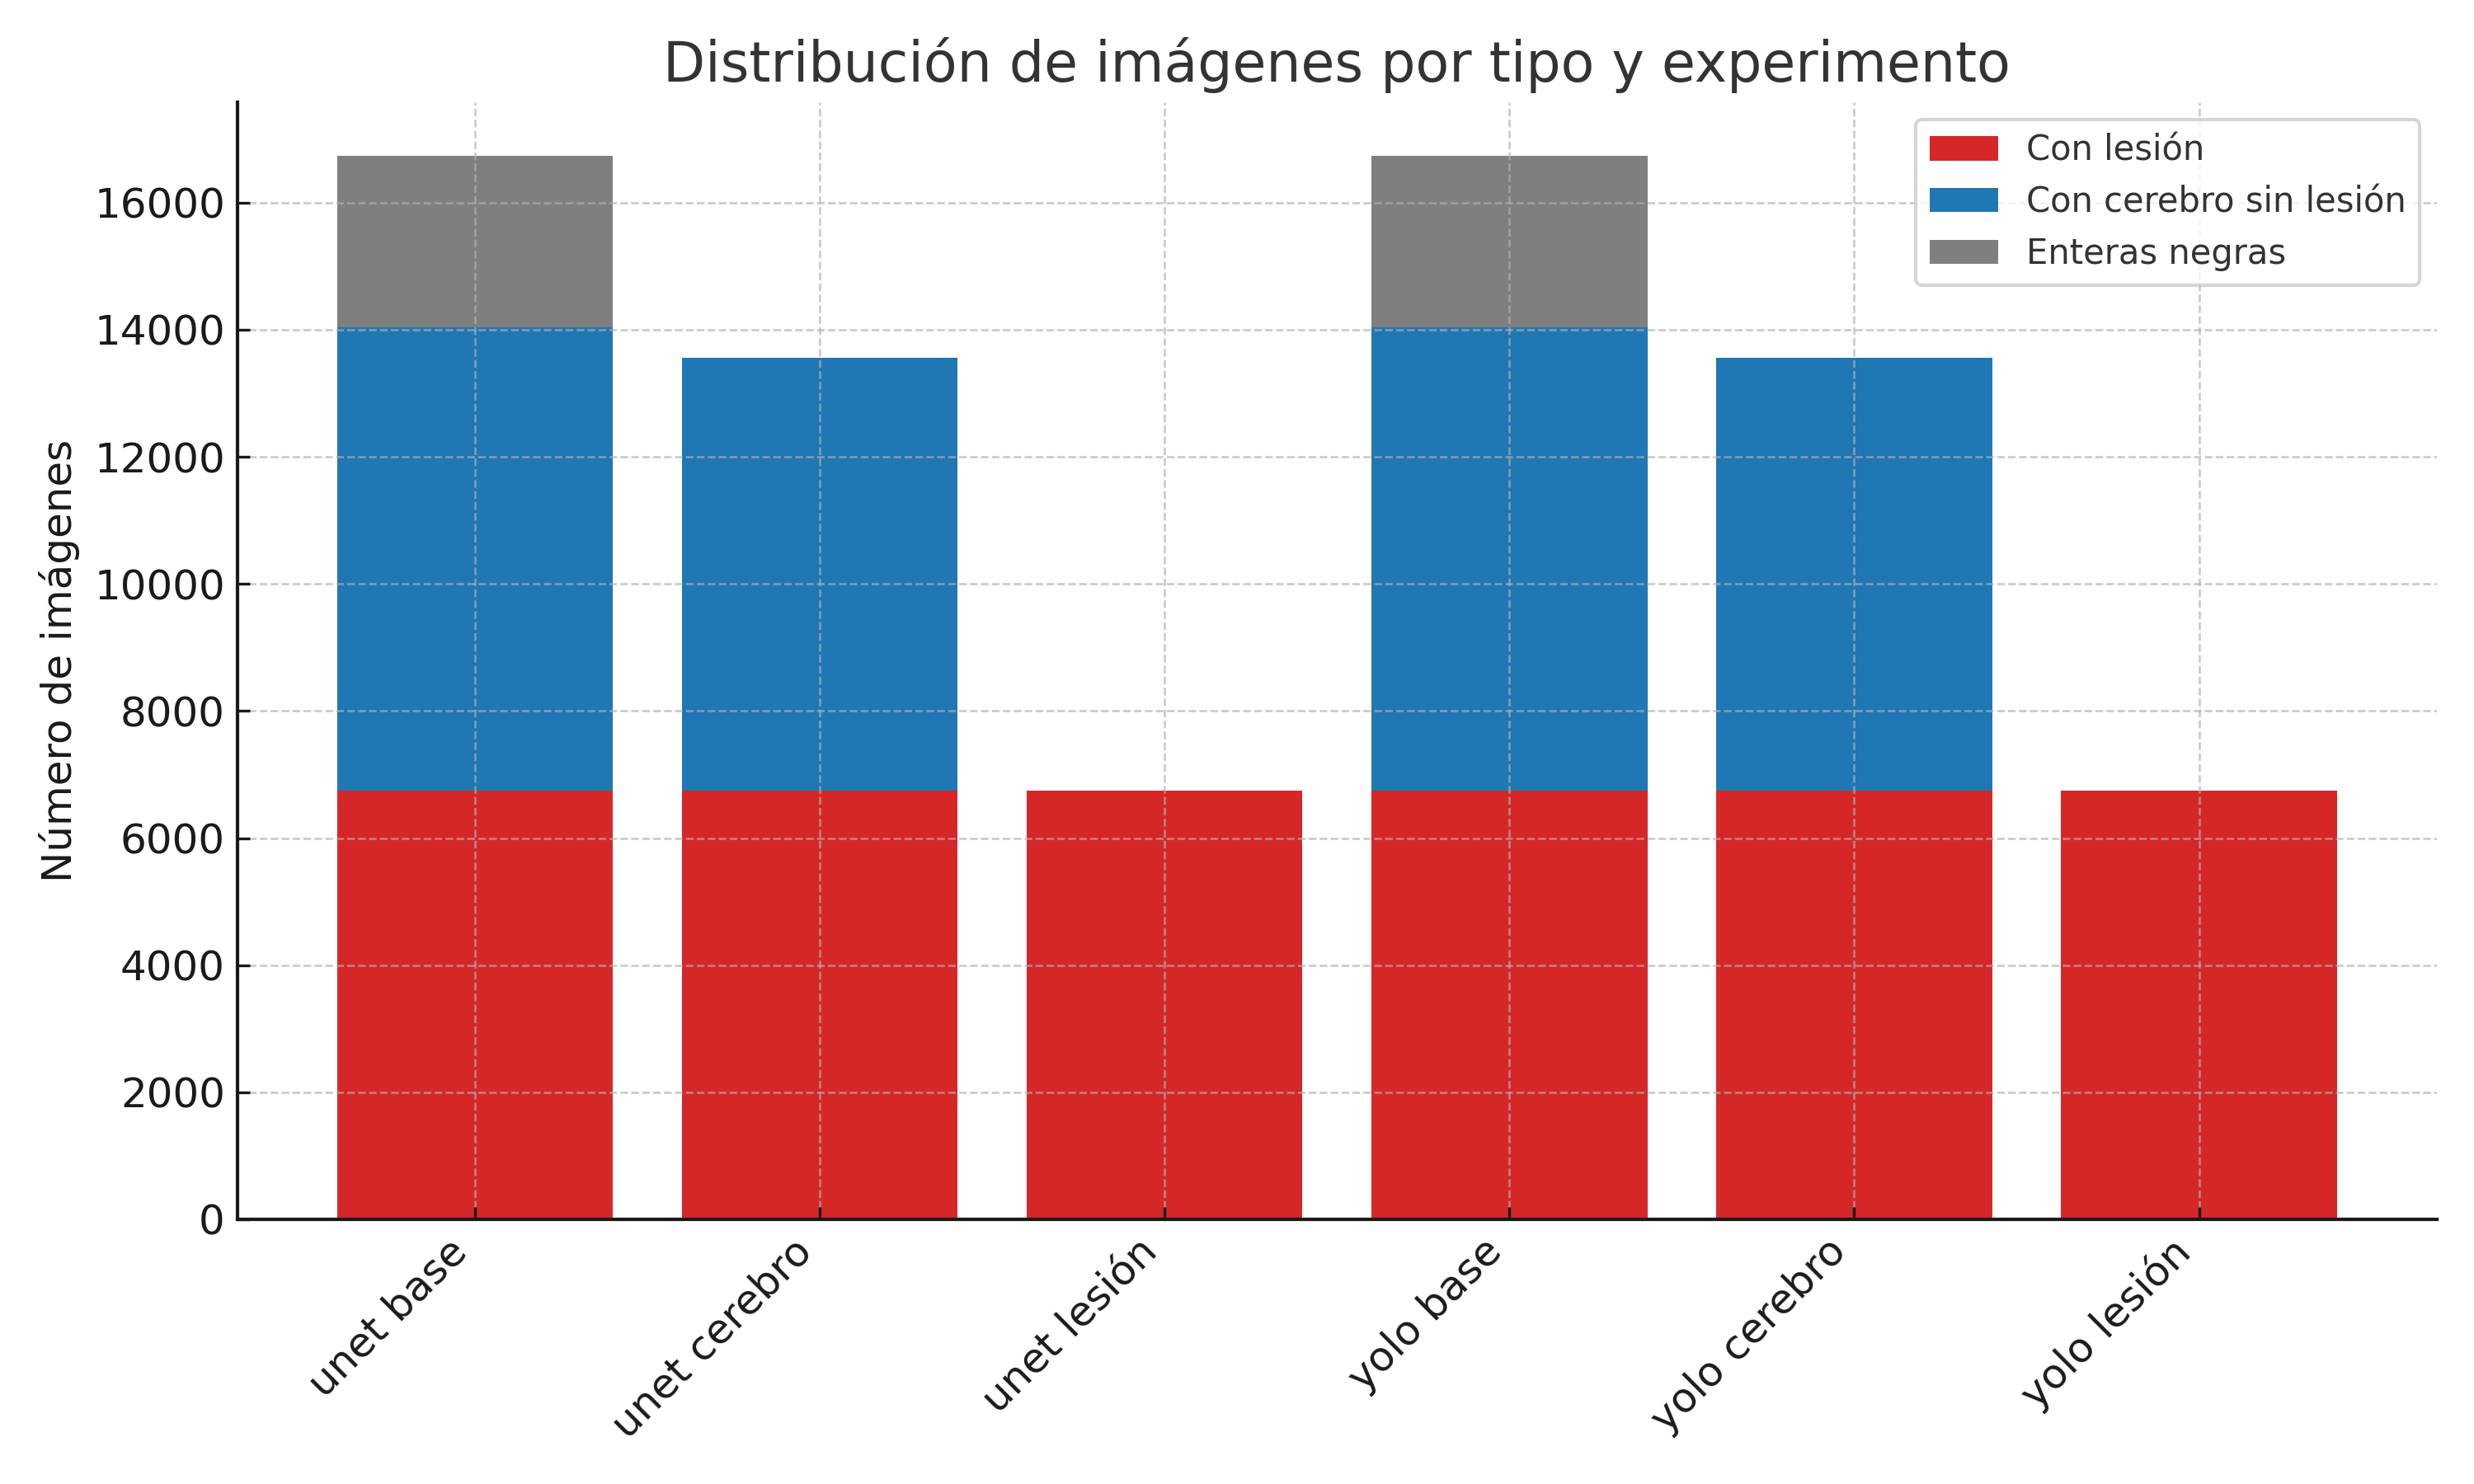
\includegraphics[width=\linewidth]{imgs/metodologia/dist_total.png}
        \caption{Distribución absoluta de imágenes por experimento}
        \label{fig:distribucion_absoluta}
    \end{subfigure}
    \hfill
    % Segunda subfigura: valores porcentuales
    \begin{subfigure}[b]{0.48\linewidth}
        \centering
        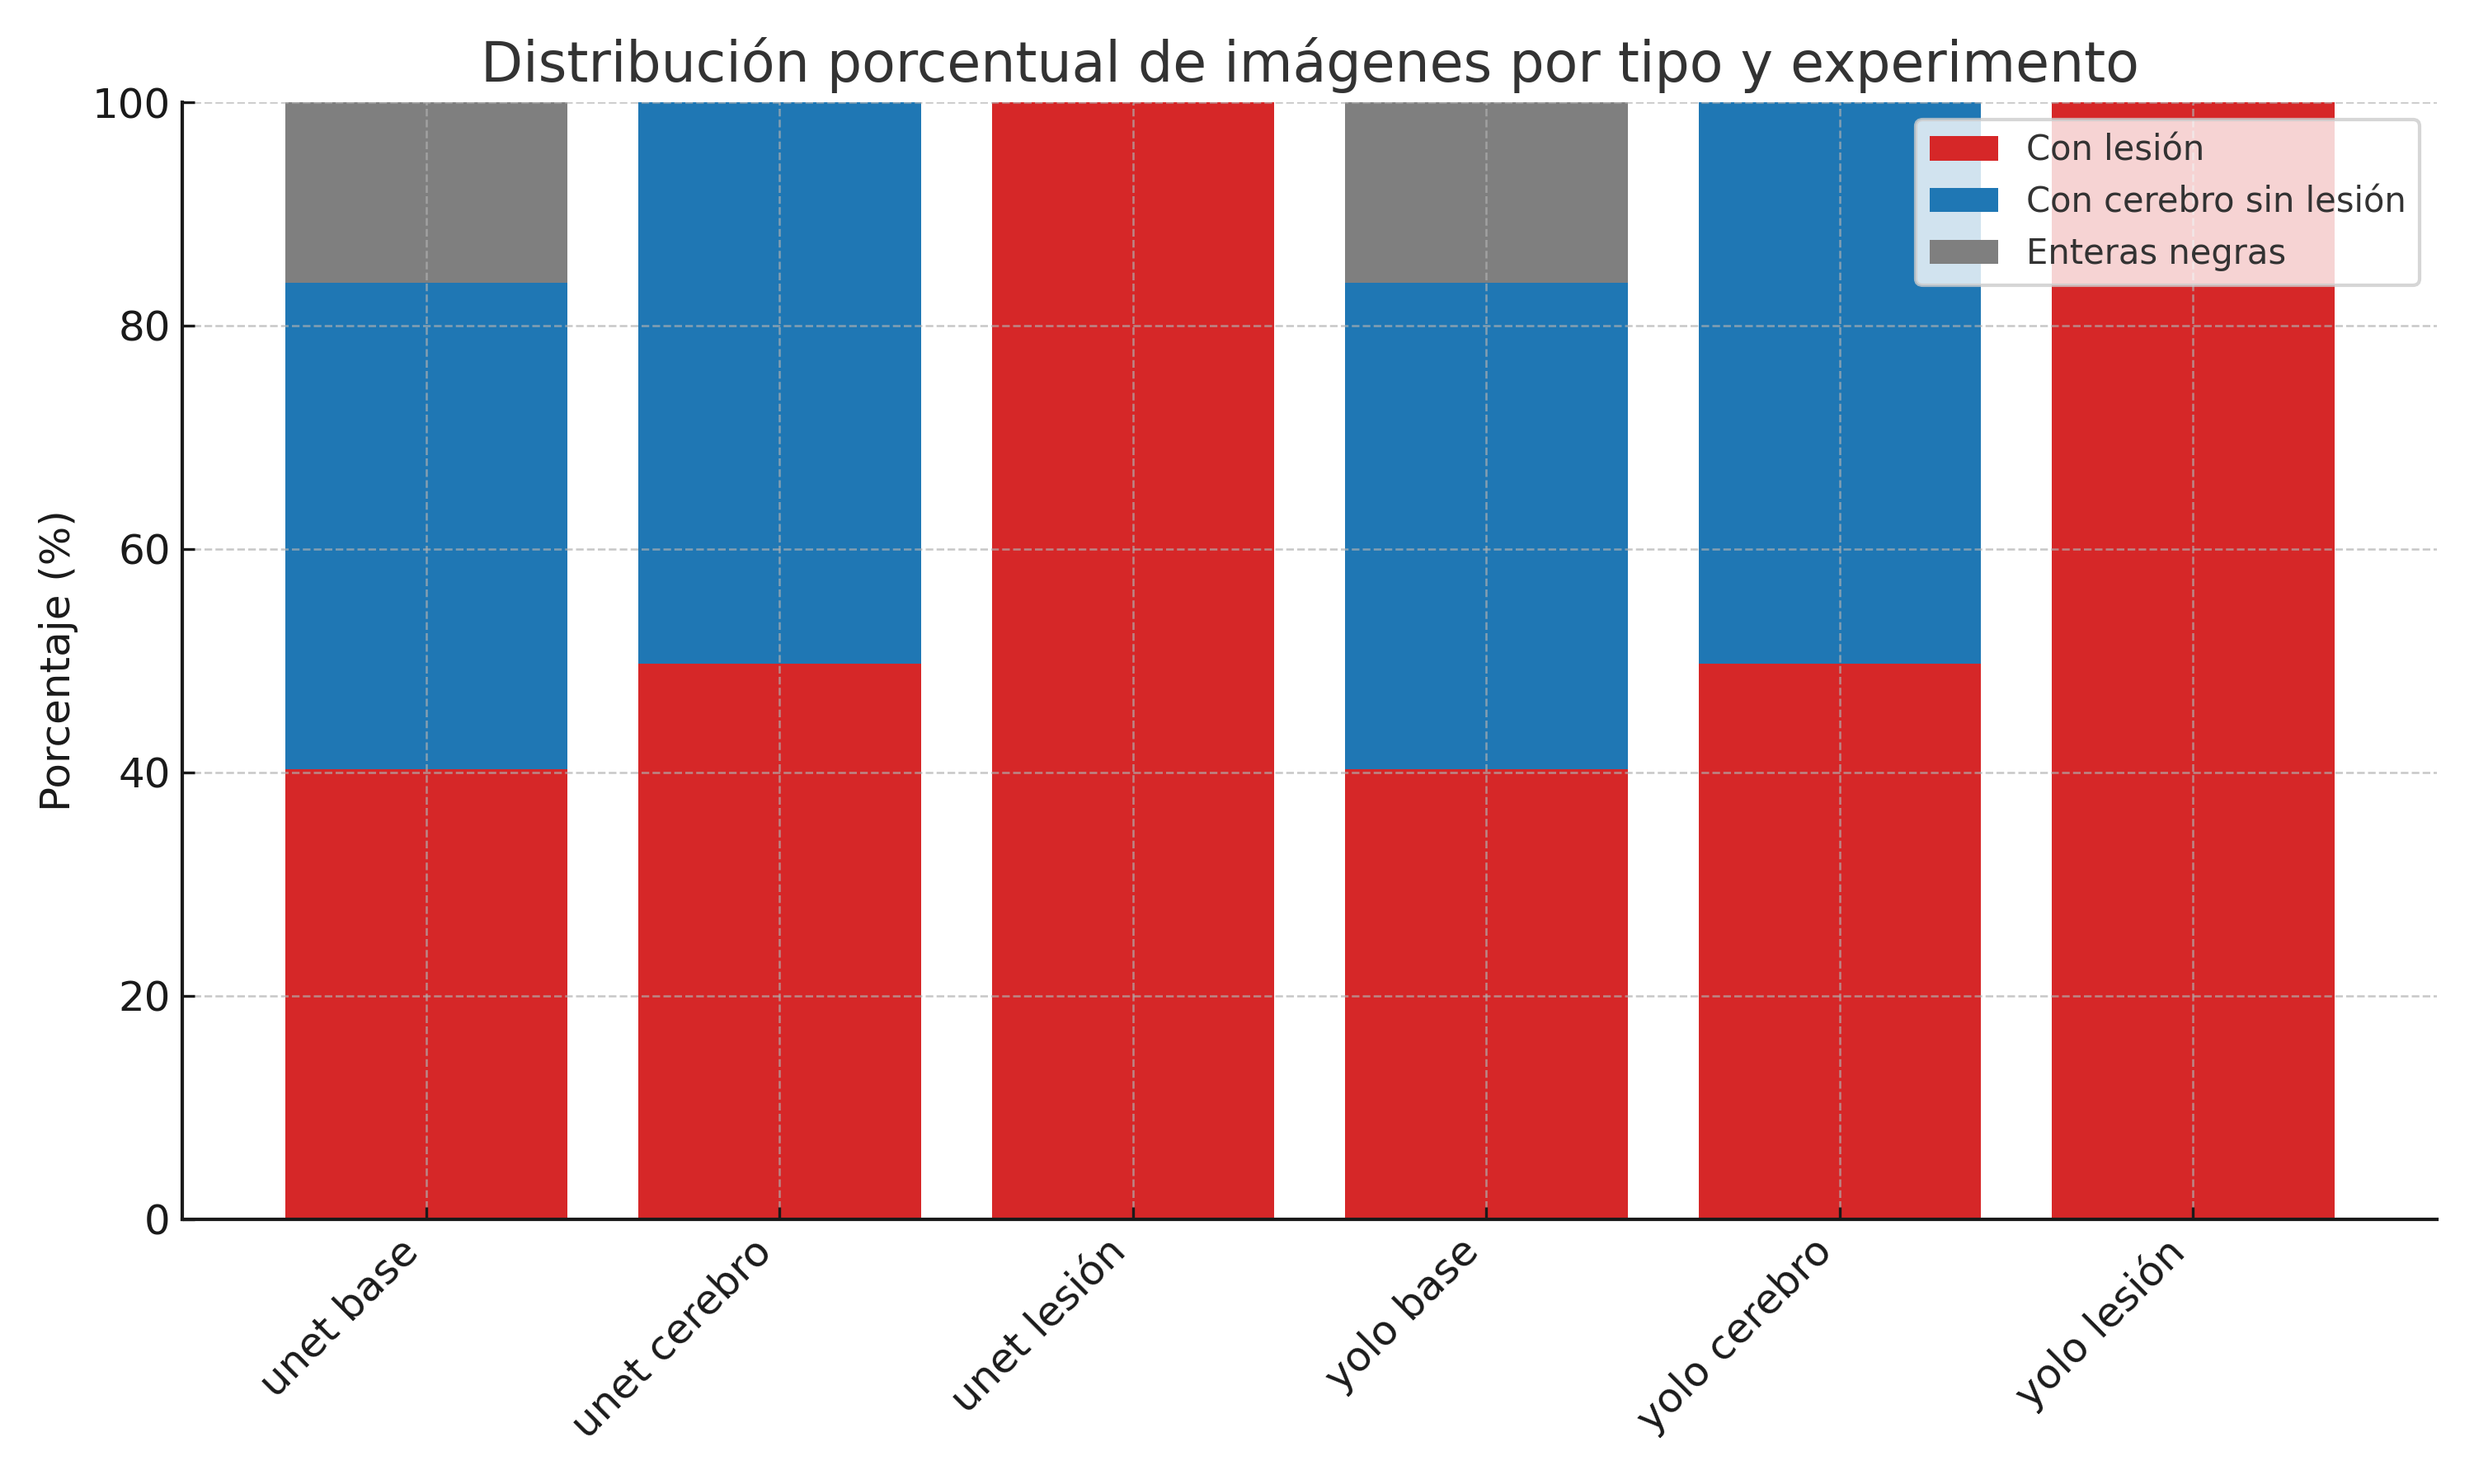
\includegraphics[width=\linewidth]{imgs/metodologia/dist_porc.png}
        \caption{Distribución porcentual de imágenes por experimento}
        \label{fig:distribucion_porcentual}
    \end{subfigure}
    \caption{Resumen de la distribución de imágenes por experimento, diferenciando entre imágenes con lesión, con cerebro sin lesión y enteras negras.}
    \label{fig:distribucion_experimentos}
\end{figure}


Se aplicó una \textbf{validación cruzada estratificada por paciente} utilizando la clase \texttt{GroupKFold} de la biblioteca \texttt{scikit-learn}, la cual garantiza que todos los cortes pertenecientes a un mismo paciente estén en un único subconjunto por \textit{fold}. Esto evita fugas de información y asegura que la distribución de pacientes sea equilibrada entre los distintos pliegues. Los resultados obtenidos en cada \textit{fold} fueron agregados mediante la media y desviación estándar de las métricas descritas al final de este capítulo, proporcionando una estimación más robusta y representativa del rendimiento de los modelos entrenados.


\subsection{Flujo de preprocesado}
Seleccionados el tipo de corte y la modalidad de las imágenes, el siguiente paso es describir el flujo de preprocesado, que tiene como objetivo generar conjuntos de datos 2D a partir de las imágenes originales en formato NIfTI adaptando el formato de salida según el tipo de red neuronal empleada. El flujo general se describe a continuación:

\begin{enumerate}
    \item \textbf{Lectura de imágenes:} se inicia con la lectura de los volúmenes de imagen y sus correspondientes máscaras de segmentación.
    \item \textbf{División del conjunto de datos:} los pacientes se dividen en tres subconjuntos mutuamente excluyentes: entrenamiento, validación y prueba. Esta división garantiza que no exista solapamiento de datos entre fases, evitando así correlaciones intrapaciente que puedan sesgar los resultados.
    \item \textbf{Selección de slices:} de cada volumen se extraen cortes axiales bidimensionales. La estrategia de selección puede variar según las descritas anteriormente.
    \item \textbf{Decisión sobre la aplicación de super-resolución (SR):}     en este punto, se determina si se aplicará o no un modelo de super-resolución. Esta decisión depende del experimento configurado.
        \begin{itemize}
            \item \textbf{Si no se aplica SR:} las imágenes y máscaras continúan directamente hacia el proceso de normalización.
            \item \textbf{Si se aplica SR:} se aplica el modelo FSRCNN únicamente a las imágenes FLAIR, con el objetivo de mejorar su resolución espacial. Las máscaras, por su naturaleza binaria o categórica, se reescalan mediante interpolación para evitar artefactos y preservar las clases originales.
        \end{itemize}
    \item \textbf{Normalización:} las imágenes FLAIR se normalizan a un rango de intensidades estándar $[0,255]$, y se redimensionan del tamaño original ($182 \times 218$) a un tamaño uniforme ($340 \times 340$ píxeles), adaptándose a los requisitos de entrada de las redes neuronales.
    \item \textbf{Binarización:} en el caso de las máscaras, el rango de intensidades se convierte a 0 (fondo negro) o 255 (lesión con píxeles blancos).
    \item \textbf{Guardado:} finalmente, tanto las imágenes como sus máscaras procesadas se almacenan en directorios separados según su propósito (entrenamiento, validación o prueba). En el caso de YOLO, las máscaras también se convierten a formato de anotación compatible (\textit{bounding boxes}) en archivos de texto.
\end{enumerate}

%\begin{figure}
%    \centering
%    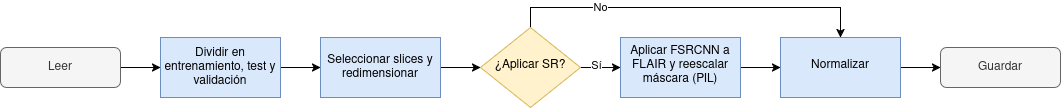
\includegraphics[width=\textwidth]{imgs/preprocess.drawio.png}
%    \caption{Diagrama de flujo del proceso de preprocesado de imágenes.}
%    \label{fig:Flujo de preprocesado}
%\end{figure}

\subsection{Estrategia de selección de imágenes}
Para maximizar el aprovechamiento de los datos y analizar el impacto de distintas formas de selección de imágenes, se han definido tres estrategias distintas para la extracción de cortes axiales a partir de los volúmenes tridimensionales:

\begin{itemize}
    \item \textbf{Base:} se incluyen todos los cortes axiales de cada volumen, sin aplicar ningún filtrado. Esta estrategia sirve como línea base para comparar el rendimiento de modelos entrenados con el conjunto completo de datos disponibles, incluyendo cortes sin lesión visible.

    \item \textbf{Lesion:} se seleccionan únicamente aquellos cortes cuya máscara contiene lesión. Esta estrategia elimina los slices vacíos que no aportan información relevante para la tarea de segmentación, reduciendo el ruido de fondo y el desbalance entre clases.

    \item \textbf{Cerebro:} se seleccionan cortes que contengan al menos una estructura cerebral visible, independientemente de si presentan lesión o no. Esta estrategia busca entrenar modelos que aprendan a segmentar el cerebro en general, lo cual es útil para tareas de segmentación más amplias que van más allá de las lesiones específicas.
\end{itemize}

Estas estrategias se aplican de forma programática durante el preprocesado, asegurando que cada imagen FLAIR extraída se acompaña de su correspondiente máscara binaria de segmentación. La comparación del rendimiento de los modelos entrenados con cada estrategia permite evaluar el impacto que tiene el tipo de datos suministrado sobre la capacidad del modelo para detectar y segmentar correctamente las lesiones de esclerosis múltiple.

\subsection{Métricas utilizadas}

Para evaluar el rendimiento de los modelos de segmentación entrenados en este trabajo, se han empleado métricas clásicas de segmentación binaria ampliamente utilizadas en el ámbito de la segmentación médica. Estas métricas permiten cuantificar tanto la precisión general del modelo como su comportamiento específico al identificar regiones lesionadas, que en este caso constituyen la clase positiva. Las métricas utilizadas son las siguientes:

\begin{itemize}
    \item \textbf{Índice de Jaccard (IoU):} también conocido como \textit{Intersection over Union}, mide la superposición entre la predicción y la máscara real. Se define como:
    \[
    IoU = \frac{TP}{TP + FP + FN}
    \]
    donde \(TP\) son los píxeles correctamente clasificados como lesión, \(FP\) son los falsos positivos y \(FN\) los falsos negativos.

    \item \textbf{Coeficiente de Dice (Dice Score):} métrica similar al IoU pero más sensible a clases desbalanceadas, ampliamente utilizada en segmentación médica:
    \[
    Dice = \frac{2TP}{2TP + FP + FN}
    \]
    En este trabajo, también se ha utilizado como métrica principal de referencia.

    \item \textbf{Precisión (Precision):} mide la proporción de verdaderos positivos sobre el total de predicciones positivas:
    \[
    Precision = \frac{TP}{TP + FP}
    \]
    Es útil para valorar la exactitud del modelo evitando predicciones incorrectas.

    \item \textbf{Sensibilidad (Recall):} mide la capacidad del modelo para detectar correctamente las regiones lesionadas reales:
    \[
    Recall = \frac{TP}{TP + FN}
    \]

    \item \textbf{Tiempo de inferencia:} se ha medido el tiempo medio de predicción por imagen, en segundos, con el objetivo de valorar la viabilidad del modelo en entornos clínicos reales. Esta métrica no afecta directamente a la calidad de la segmentación, pero es crítica para su aplicabilidad práctica.
\end{itemize}

El conjunto de métricas seleccionadas permite una evaluación completa del sistema, considerando tanto su capacidad de detectar correctamente las lesiones como de evitar falsos positivos, además de su eficiencia computacional.

\subsection{Entrenamiento}
El proceso de entrenamiento de los modelos de segmentación se ha llevado a cabo adaptando la arquitectura y configuración a las características específicas del problema. En el caso de U-Net, se ha utilizado un codificador basado en ResNet34 preentrenado con el conjunto de imágenes \textit{ImageNet}, lo que permite transferir conocimiento aprendido en tareas generales de visión por computador y acelerar la convergencia del modelo. La entrada a la red consiste en imágenes unicanal correspondientes a cortes axiales de resonancia magnética FLAIR, mientras que la salida es un mapa de segmentación con activación lineal, sobre el cual se aplica una función sigmoide en la fase de evaluación.

La función de pérdida utilizada combina dos componentes complementarios: la \texttt{Binary Cross-Entropy} (BCE), que penaliza errores píxel a píxel, y la \texttt{Dice Loss}, que favorece la superposición espacial entre predicción y máscara. La combinación se expresa como:

\begin{equation}
\mathcal{L}(x, y) = \text{BCEWithLogitsLoss}(x, y) + \left(1 - \frac{2 \sum_i \sigma(x_i) y_i + \varepsilon}{\sum_i \sigma(x_i) + \sum_i y_i + \varepsilon}\right)
\end{equation}

donde \(x\) representa la salida cruda del modelo (logits), \(\sigma(x)\) es la función sigmoide aplicada a cada valor de salida, \(y\) es la máscara binaria de referencia, y \(\varepsilon = 10^{-5}\) es un término de suavizado para evitar inestabilidades numéricas. La optimización del modelo se realiza mediante el algoritmo \texttt{Adam}, ampliamente utilizado por su eficiencia y capacidad de adaptación a diferentes escalas de gradientes. Para mejorar la capacidad generalizadora del modelo, se ha incorporado un plan de ajuste dinámico de la tasa de aprendizaje mediante la política \texttt{ReduceLROnPlateau}, que reduce el valor del \textit{learning rate} cuando la pérdida de validación no mejora durante varias épocas consecutivas.

 %Se ha utilizado el optimizador por defecto (\texttt{SGD}) y un conjunto de hiperparámetros estándar proporcionado por la configuración oficial de Ultralytics. En la Tabla~\ref{tab:yolo-defaults} se presentan los valores por defecto más relevantes.

% \begin{table}
% \centering
% \caption{Principales hiperparámetros por defecto por utilizados por YOLO (Ultralytics).}
% \label{tab:yolo-defaults}
% \begin{tabular}{ll}
% \toprule
% \textbf{Parámetro} & \textbf{Valor por defecto} \\
% \midrule
% Épocas & 100 \\
% Tamaño de batch & 16 \\
% Tamaño de imagen (\texttt{imgsz}) & 640 \\
% Tasa de aprendizaje inicial (\texttt{lr0}) & 0.01 \\
% Optimización & SGD (momentum = 0.937, weight decay = 0.0005) \\
% Pérdidas & box = 7.5,\quad cls = 0.5,\quad dfl = 1.5 \\
% Warmup epochs & 3.0 \\
% Patience (early stopping) & 100 \\
% Precisión mixta (\texttt{AMP}) & Activada \\
% Aumento de datos (Mosaic, multiscale) & Desactivado \\
% Scheduler & Cosine (opcional) \\
% \bottomrule
% \end{tabular}
% \end{table}

El entrenamiento de YOLO se realiza mediante la combinación de varias funciones de pérdida: localización (coordenadas de \textit{bounding boxes}), clasificación de clase y segmentación. Por otra parte, se ha procurado mantener la coherencia en los principales hiperparámetros de entrenamiento entre ambos modelos con el fin de garantizar una comparación equitativa y controlada. En particular, se ha fijado una tasa de aprendizaje inicial de $0.001$, un tamaño de batch de 16 y un total de 50 épocas de entrenamiento tanto para U-Net como para YOLO. Este ajuste ha sido necesario para igualar las condiciones experimentales y observar el impacto de la arquitectura y el preprocesado, minimizando el efecto de otros factores externos.
La Tabla~\ref{tab:hiperparametros} resume los principales hiperparámetros utilizados en ambos casos.

\begin{table}[h]
\centering
\caption{Comparación de hiperparámetros entre U-Net y YOLO.}
\label{tab:hiperparametros}
\begin{tabular}{lcc}
\toprule
\textbf{Parámetro} & \textbf{U-Net} & \textbf{YOLO} \\
\midrule
Tamaño de batch       & 16                & 16 \\
Épocas                & 50                & 50 \\
Tasa de aprendizaje   & 0.001             & 0.01 \\
Optimizador           & Adam              & SGD \\
Scheduler             & ReduceLROnPlateau & Cosine (opcional) \\
Función de pérdida    & BCE + Dice        & Box + Class + DFL \\
Precisión mixta (AMP) & Sí                & Sí \\
Semilla aleatoria     & 42                & 42 \\
Confianza             & 0.5               & 0.5 \\
Aumento de datos      & No                & No \\
\bottomrule
\end{tabular}
\end{table}


\end{document}